\subsection{Second-order plant}

If the electrical dynamics are not neglected, the motor is no longer a
first-order plant. With armature inductance \(L_a\), armature resistance
\(R_a\), inertia \(J\), viscous friction \(b\), and motor constant \(K_m\), the
continuous-time transfer function becomes
\begin{equation}
  G(s)=
  \frac{K_m}
       {L_aJs^2+\left(L_ab+R_aJ\right)s+\left(R_ab+K_m^2\right)} .
  \label{eq:second-order-continuous-transfer}
\end{equation}
After zero-order-hold discretisation this is written as
\begin{equation}
  G(z)=\frac{b_1z+b_0}{z^2+a_1z+a_0}.
  \label{eq:second-order-discrete-transfer}
\end{equation}
The adaptive estimator therefore has four parameters instead of two. Its
regression vector is
\begin{equation}
  \varphi(k)=
  \begin{bmatrix}
    -y(k-1) & -y(k-2) & u(k-1) & u(k-2)
  \end{bmatrix},
  \label{eq:second-order-regressor}
\end{equation}
and the controller is no longer the incremental PI law of
\eqref{eq:incremental-pi}. It becomes an RST controller whose parameters are
computed at each sampling instant from the Diophantine system given in
equation 7.16 of the reader.

The decisive point is not the algebraic increase from two to four parameters,
but the sampling time. For
\[
  K_m=0.05,\quad
  J=\SI{0.001}{kg.m^2},\quad
  b=0.0005,\quad
  L_a=\SI{2}{mH},\quad
  R_a=\SI{2}{\ohm},
\]
the continuous poles are \(-998.7\,\si{s^{-1}}\) for the electrical mode and
\(-1.75\,\si{s^{-1}}\) for the mechanical mode. The electrical time constant
is therefore about \(\SI{1}{ms}\). Table~\ref{tab:second-order-zoh-values}
shows the exact ZOH discretisation for the slow sampling time used on the
hardware and for a sampling time that resolves the electrical pole.

\begin{scripttable}
  \centering
  \caption{Exact ZOH parameters of the second-order motor model.}
  \label{tab:second-order-zoh-values}
  \begin{tabular}{rrrrrrl}
    \toprule
    \(T\) & \(a_1\) & \(a_0\) & \(b_1\) & \(b_0\) & \multicolumn{2}{c}{\(z\)-poles} \\
    \midrule
    \(\SI{80}{ms}\) & \(-0.8692\) & \(0.000000\) & \(1.8467\) & \(0.0218\) & \(0.8692\) & \(0\) \\
    \(\SI{2}{ms}\)  & \(-1.1322\) & \(0.1352\)   & \(0.0284\) & \(0.0148\) & \(0.9965\) & \(0.1357\) \\
    \bottomrule
  \end{tabular}
\end{scripttable}

At \(T=\SI{80}{ms}\), the electrical pole is mapped to \(z=0\). It has fully
decayed between two samples. Two of the four parameters then no longer
contribute independent information to the measured output, the regressor loses
rank, and the estimate drifts along the non-identifiable direction. The model
is not merely over-parameterised at this sampling time; it is structurally not
identifiable. Figure~\ref{fig:second-order-identifiability} shows this loss of
information by plotting the magnitude of the smaller discrete pole against the
sampling time.

\begin{figure}[htbp]
  \centering
  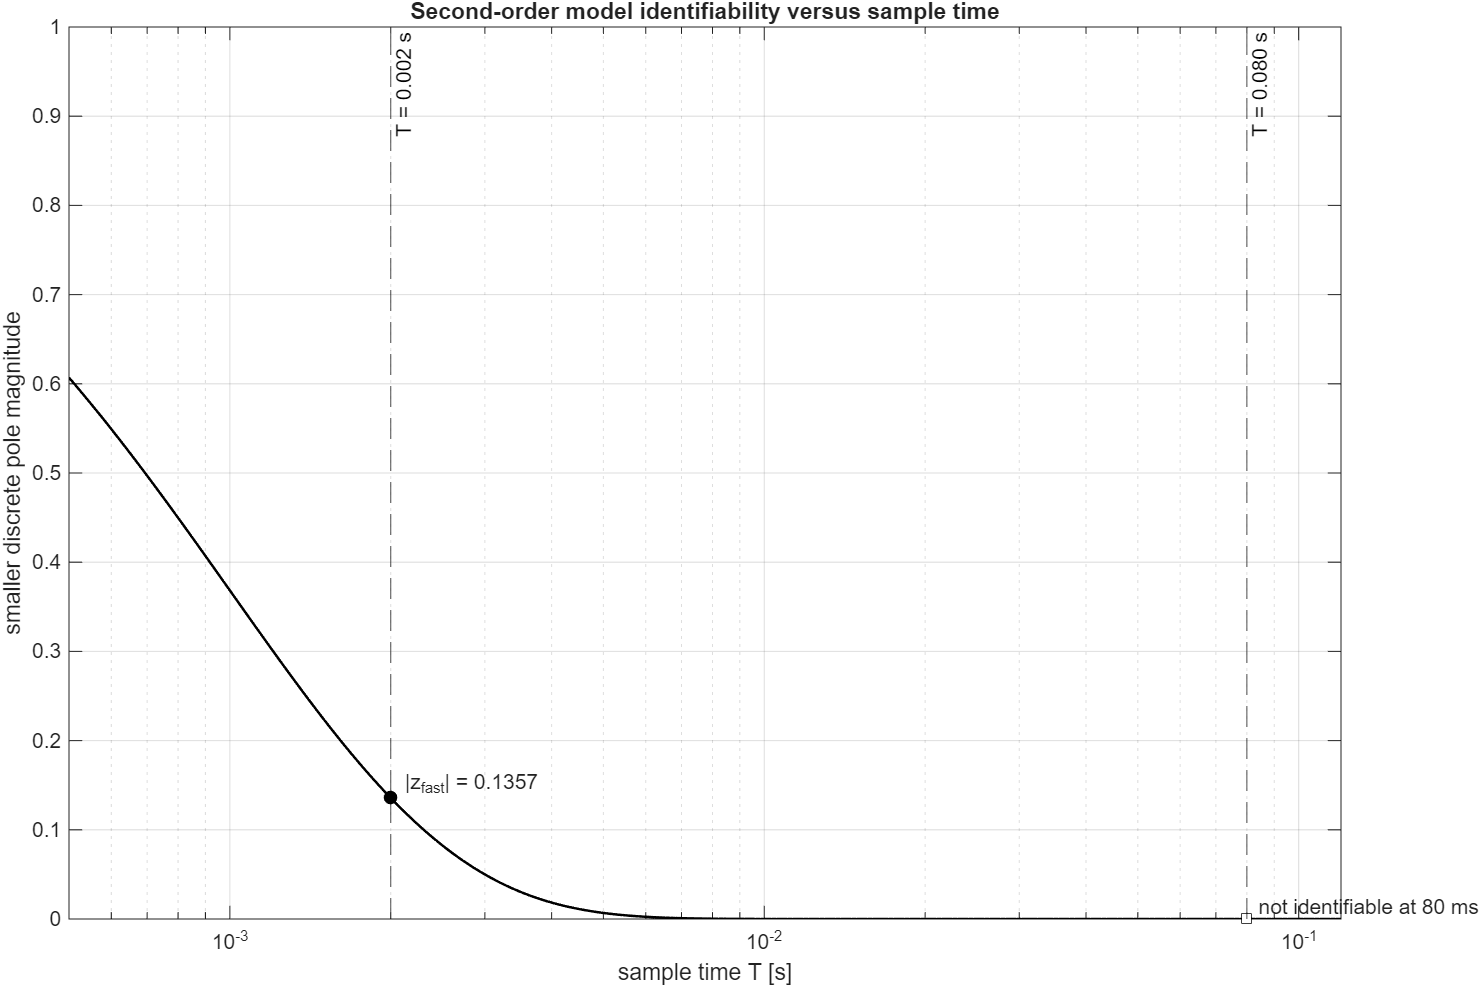
\includegraphics[width=0.82\linewidth]{../img/identifiability_T.png}
  \caption{Magnitude of the smaller ZOH pole of the second-order motor model
  as a function of the sampling time.}
  \label{fig:second-order-identifiability}
\end{figure}

The consequence is easy to overlook in practice. At \(T=\SI{80}{ms}\) the
closed loop can still follow the reference stably, even though the parameter
estimate cannot converge under that sampling. A stable closed loop is therefore
not evidence of successful identification. The RST controller only needs
certain combinations of the parameters, not their individual values.

The working design uses \(T=\SI{2}{ms}\). Persistent excitation is supplied by
adding a PRBS dither to the manipulated variable. The dither is not added to
the reference: a controller that is asked to track a fast rectangular reference
drives the actuator into saturation, and an identification experiment with a
saturating actuator is worthless. Four parameters require excitation of the
corresponding order.

The estimator is used without forgetting, \(\alpha=1\). Without persistent
excitation, \(\alpha<1\) makes \(P\) grow without bound in the unexcited
directions. This covariance windup makes the estimate drift and can destabilise
the controller. In simulation, the control error grew to
\(\SI{88}{\percent}\).

Integral action is also required. Pure pole placement fixes only the poles, not
the static gain, and therefore leaves a steady-state error. The simulated value
was \(\SI{7.8}{\percent}\). The controller denominator is therefore chosen as
\begin{equation}
  c(z)=(z-1)(z+c_0),
  \label{eq:second-order-integrator}
\end{equation}
which gives \(T(1)=1\).

The desired closed-loop polynomial is
\begin{equation}
  q(z)=z(z-0.1357)(z-0.9608)^2 .
  \label{eq:second-order-desired-polynomial}
\end{equation}
The fast electrical pole is deliberately left in place. If instead
\[
  q(z)=(z-0.9608)^4
\]
is demanded, the design slows the electrical pole by a factor of 50. The
controller must then invert the fast plant dynamics and becomes unstable
itself; the controller pole is at \(|z|=2.66\). Behind a saturation limit, such
a controller necessarily diverges. The design rule is therefore to leave modes
that are much faster than the desired bandwidth where they are.

The validation run with \(T=\SI{2}{ms}\) is summarised in
Figure~\ref{fig:second-order-simulation}. All four parameters converge to
their true ZOH values. In the window \(t=\SIrange{3}{4}{s}\), all four
parameters lie within \(\SI{0.65}{\percent}\) relative error of their true ZOH
values.

\begin{scripttable}
  \centering
  \caption{Validated second-order parameter estimates at \(T=\SI{2}{ms}\).}
  \label{tab:second-order-validated-estimates}
  \begin{tabular}{lrrr}
    \toprule
    Parameter & Estimated, \(t=\SIrange{3}{4}{s}\) & True & Absolute error \\
    \midrule
    \(a_1\) & \(-1.131310\) & \(-1.132176\) & \(8.66\times10^{-4}\) \\
    \(a_0\) & \( 0.134337\) & \( 0.135200\) & \(8.63\times10^{-4}\) \\
    \(b_1\) & \( 0.028348\) & \( 0.028362\) & \(1.49\times10^{-5}\) \\
    \(b_0\) & \( 0.014889\) & \( 0.014832\) & \(5.71\times10^{-5}\) \\
    \bottomrule
  \end{tabular}
\end{scripttable}

The static closed-loop gain is \(T(1)=1.000\). For the step at
\(t=\SI{5.5}{s}\), the response has no
overshoot and the \(2\%\) settling time is \(\SI{0.384}{s}\). The remaining
steady-state errors in the settled windows are \(\SI{0.000}{\percent}\),
\(\SI{0.000}{\percent}\), and \(\SI{0.002}{\percent}\). The trace of \(P\)
remains bounded at 400.

\begin{figure}[htbp]
  \centering
  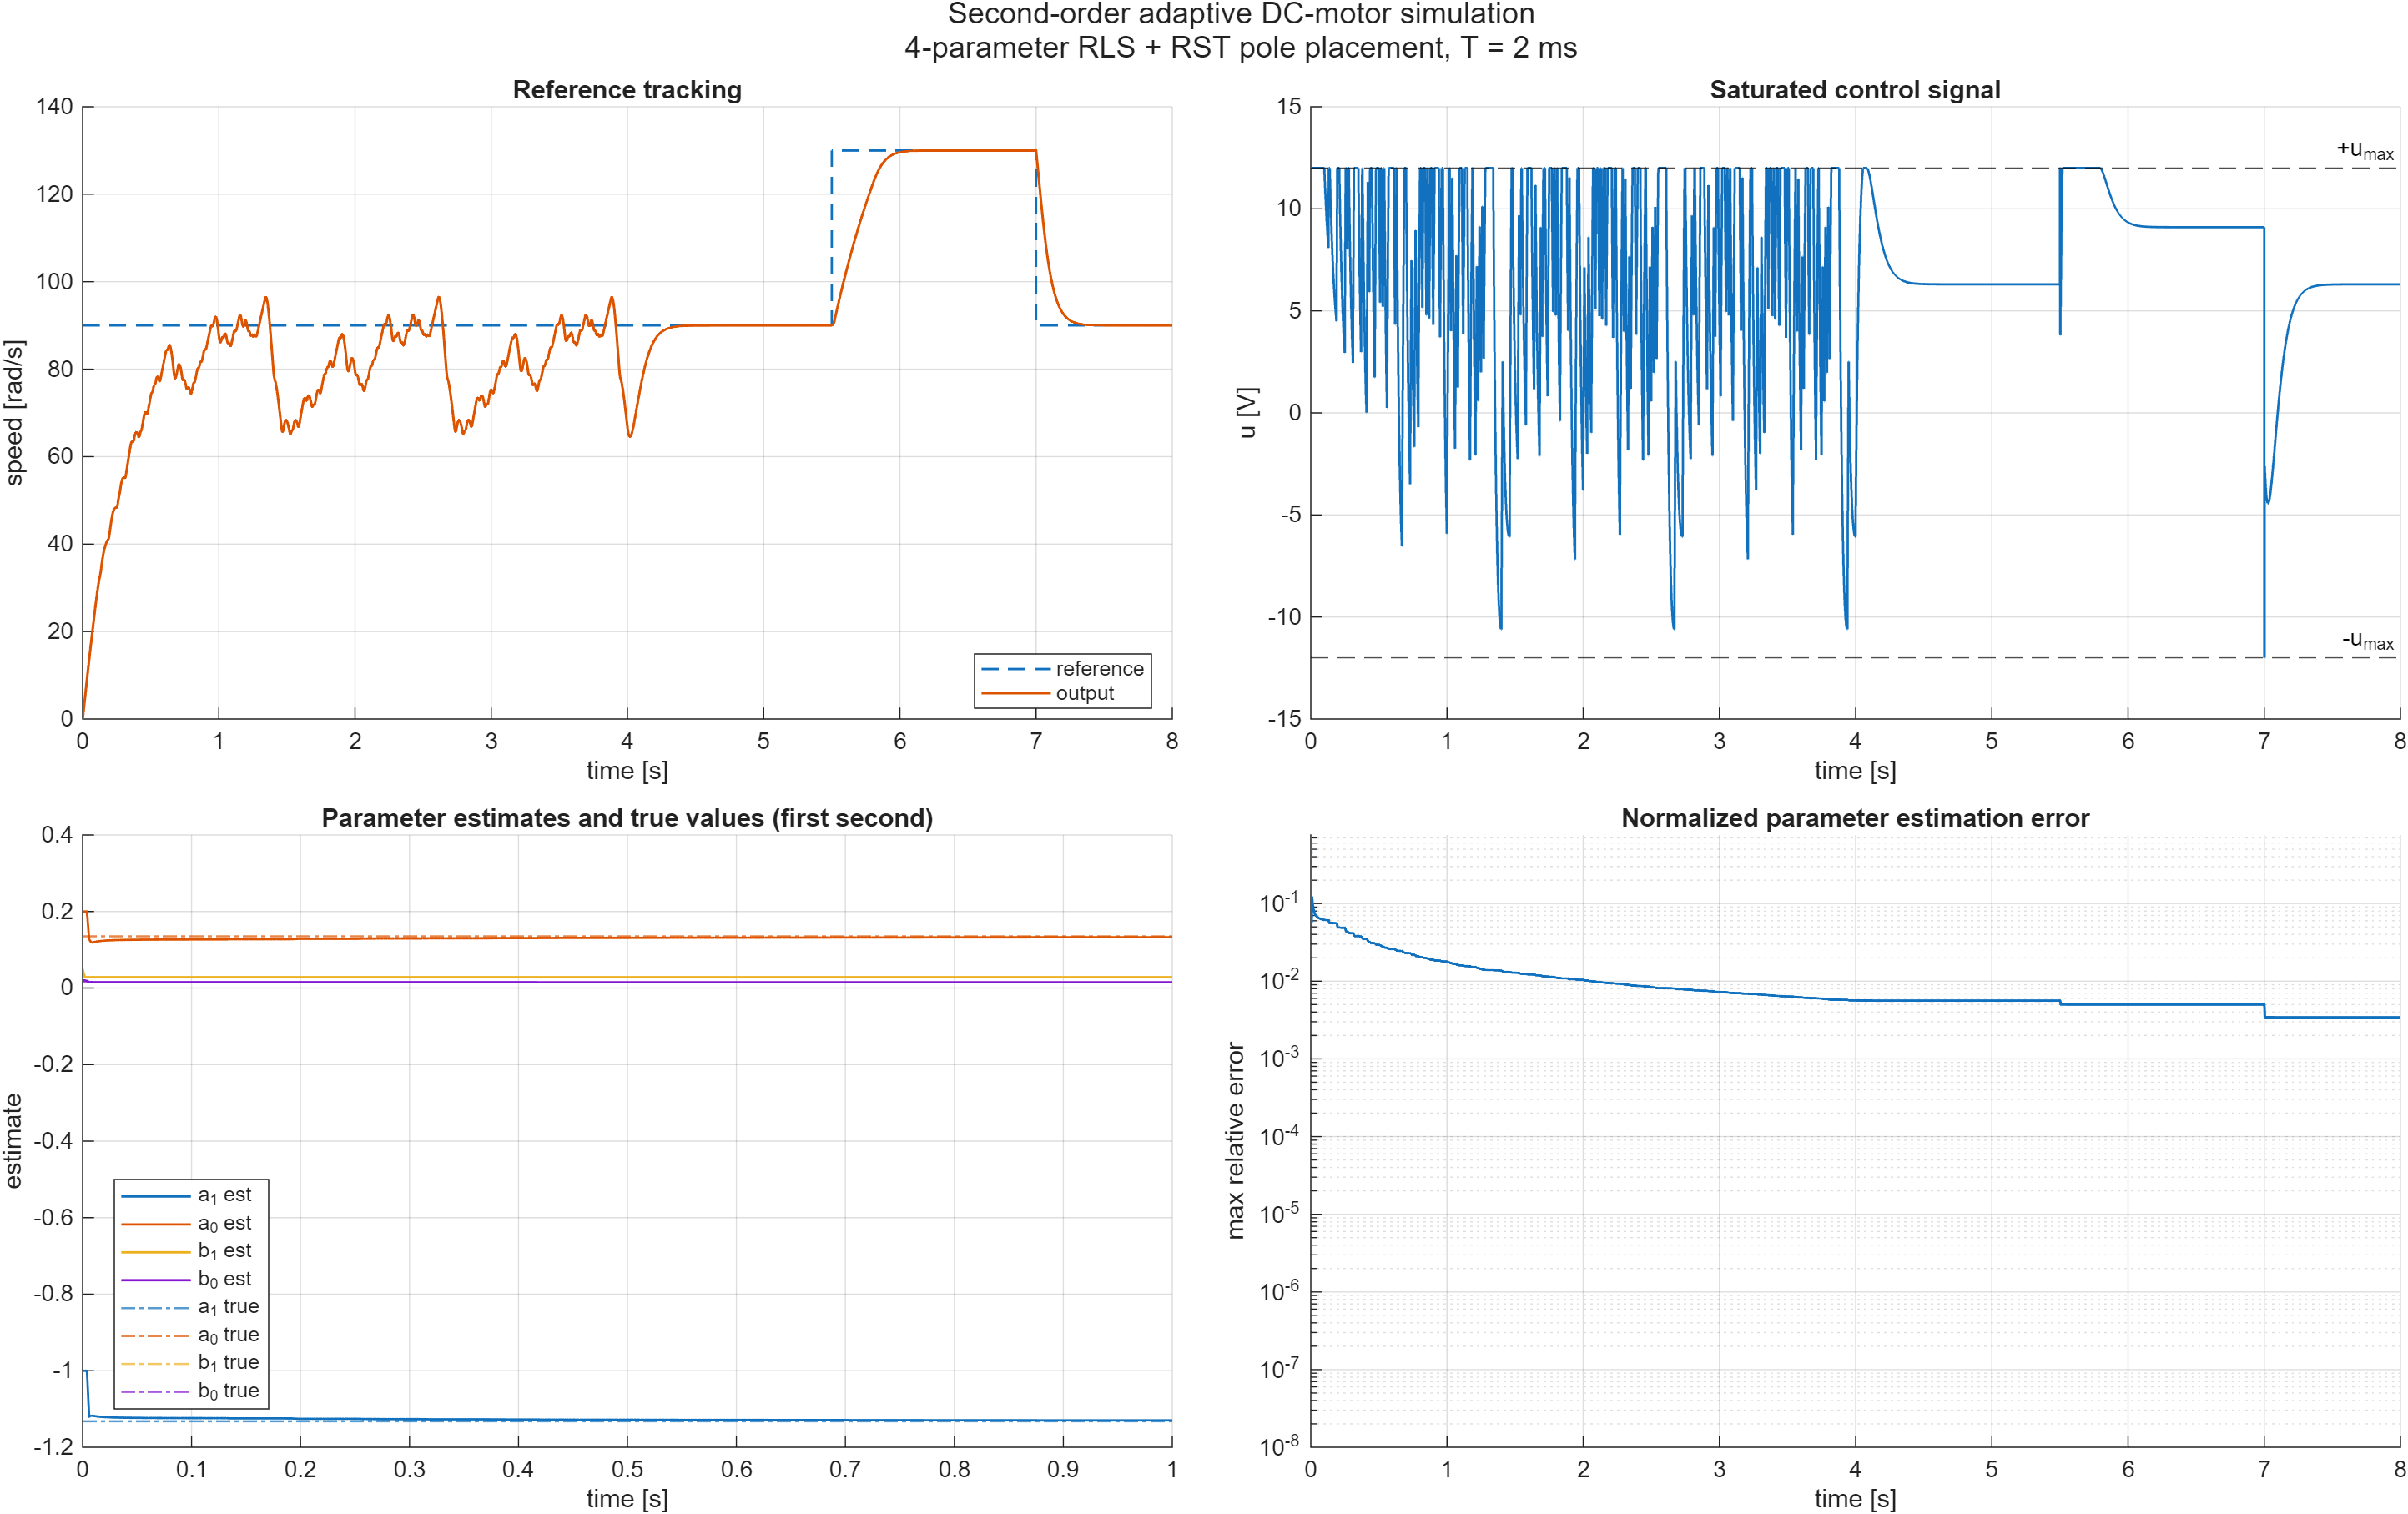
\includegraphics[width=0.82\linewidth]{../img/simulation_2nd_order.png}
  \caption{Validation run of the second-order adaptive RST controller with
  \(T=\SI{2}{ms}\), persistent excitation, integral action, and the electrical
  pole retained in the desired polynomial.}
  \label{fig:second-order-simulation}
\end{figure}

The first-order controller needs only two parameters, coarse excitation, and
\(T=\SI{80}{ms}\), and it runs on the hardware. The second-order controller
describes the plant more accurately, but it requires a sampling time that is
40 times shorter, targeted excitation, and much more care in the forgetting
factor, integral action, and pole choice. This extra effort is worthwhile only
when the electrical dynamics are relevant in the frequency range of interest.
